\section{Plataforma utilizada}
	\label{sec:AGG}
	
	Cómo se explicó Sección \ref{sec:plataforma}, es posible utilizar una FPGA de cualquier fabricante, siempre y cuando tenga determinadas características de tamaño. En este contexto se optó por utilizar la FPGA ARTY Z7-20 de Xilinx (Figura \ref{fig:FPGA}) debido a cuestiones de disponibilidad y experiencia previa con la plataforma. La misma posee 53200 Look-up-tables, 106400 Flip-Flops, 32 Buffers y 125 bloque de entrada/salida. El precio promedio de esta plataforma ronda los 300 U\$D, un precio razonable para una plataforma de nivel intermedio.	
	
	\begin{figure}[H]
		\centering
		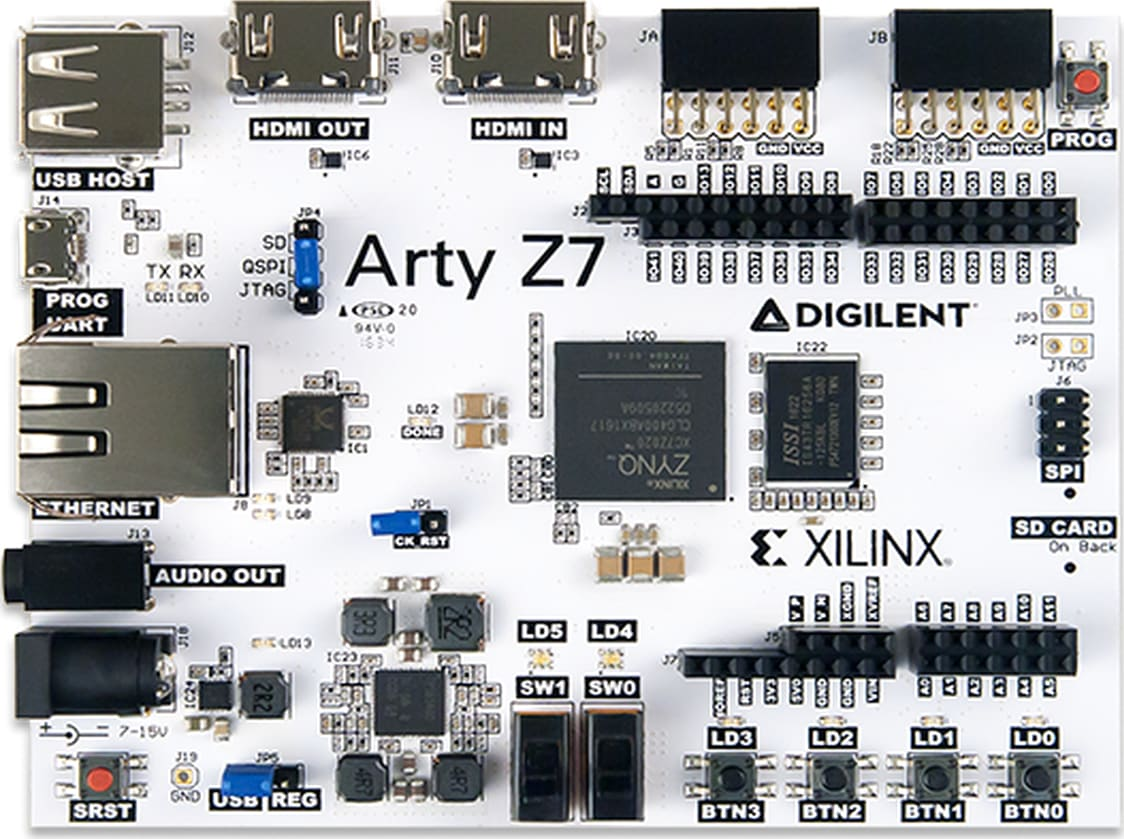
\includegraphics[width=1\textwidth]{Figuras/FPGA}
		\centering\caption{Plataforma FPGA Xilinx Arty Z7-20.}
		\label{fig:FPGA}
	\end{figure}
	
	Aunque se seleccionó una FPGA de la familia Xilinx \cite{Paper_30,Paper_36,Paper_37,Paper_40,Paper_41,Paper_47,Paper_97,Paper_104,Paper_106} y se utilizó el entorno de desarrollo integrado Vivado \cite{VIVADO,Paper_111}, por lo explicado en la Sección \ref{sec:plataforma}, el código VHDL generado por el ACG es independiente de la plataforma que se utilice. De emplearse otra familia de FPGAs, solo será necesaria una nueva asignación manual de pines de entrada y salida. De emplearse FPGAs por fuera de las familias ofrecidas por Xilinx, cómo por ejemplo Intel, puede utilizarse el entorno de desarrollo Intel Quartus \cite{QUARTUS}.
	
	Tanto el entorno de desarrollo Xilinx Vivado como el Intel Quartus incorporan herramientas para validación de la sintaxis generada por el ACG. Se utilizó la primera de ellas para generar el diagrama de bloques del sistema y analizar cada uno de los módulos y sus elementos internos. Este proceso incluye una validación de la sintaxis de todos los archivos generados por el ACG. Un análisis similar se realiza en las etapas de síntesis e implementación, detallado en profundidad en el Capítulo \ref{sec:resultados}.
	
	%La elección de una FPGA por sobre un microprocesador se debe a las ventajas expuestas en la Sección \ref{sec:FPGA} respecto a la concurrencia del sistema, mayor nivel de seguridad y facilidad para redundar el sistema. Además, los sistemas implementados en FPGA son considerados puramente hardware y no software, por lo que solamente deben cumplir los requerimientos de la norma EN 50129, especialmente el anexo F referido a FPGAs, y no la norma EN 50128 que se encarga del software. Los alcances de estas normas ya fueron explicados en la Sección \ref{sec:normas}.